\section{Hardware}
\label{sec:hardware}
An Arduino Uno with an ATmega328/P\cite{uno} is used to control the game and
hardware. All external components are connected to one or more pins of this
Arduino.

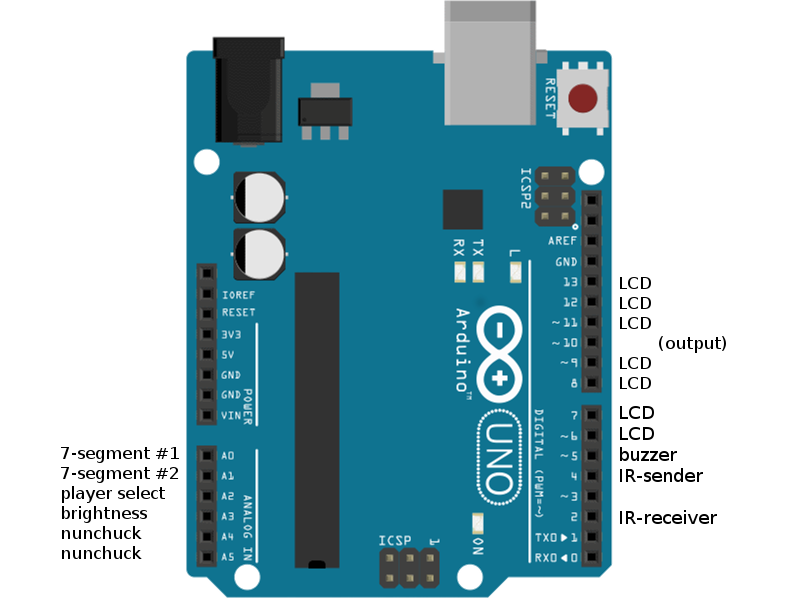
\includegraphics[width=\textwidth,height=\textheight,keepaspectratio]{res/pinmap.png}

Digital pins 0 and 1 could have been used, but are not because they are also
used for serial printing, which is useful for debugging. Pin 10 can still be
used as long it is used as an output.

\subsection{Player select}
\label{sec:playerselect}

Because it's very important to know which Arduino is player one and which one
is player two, it's possible to set the player number with a hardware DIP-
switch.

The DIP-switch is connected to an input pin with enabled pull-up resistor on
the Arduino---pin A2---and the ground. By reading the current pin state during
initialisation the Arduino knows if it should control player 1 or player 2.

In addition to selecting the right player to control, it could have been used
for IR communication. By specifying the ID of the source in each packet,
packets from the source itself can be ignord.

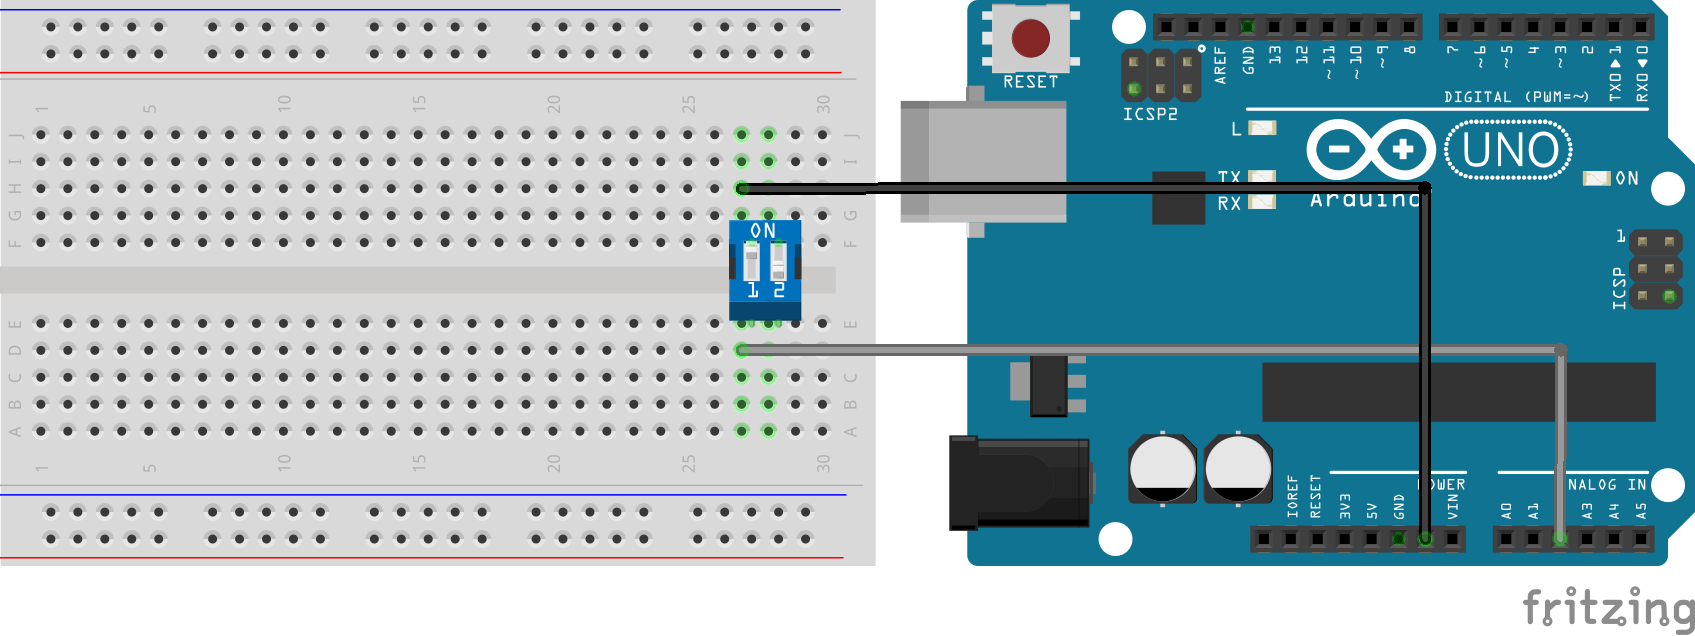
\includegraphics[width=\textwidth,height=\textheight,keepaspectratio]{res/DIP-switch.png}

\subsection{IR-communication}
\label{sec:ir-communication}

IR communication is not included in the game, but the required hardware
components \emph{are} present in the hardware package. Each Arduino Uno has its
own transmitter and receiver:

The transmitter (IR-led) has to flash with a frequency of 38kHz, since the
receiver only sees light with that frequency. This is achieved by using an
external circuit with a 555 timer to make the IR led flash, without using
timers from the ATmega chip. This circuit can be started using a digital output
pin (pin D4). A timer in the Arduino is only used to control and measure the
length of pulses.

The receiver (TSOP2138) has to be wired to a ground pin and a 5V output to
provide the receiver with power. The receiver also has an output pin, connected
to input pin D2, that will change it's voltage based on the received infrared
light. Pin D2 can trigger external pin interrupts in the Arduino. The ouput
from the receiver is low when it is recieving infrared light with the right
frequency (38 kHz) and is equal to the input voltage when it is not recieving.

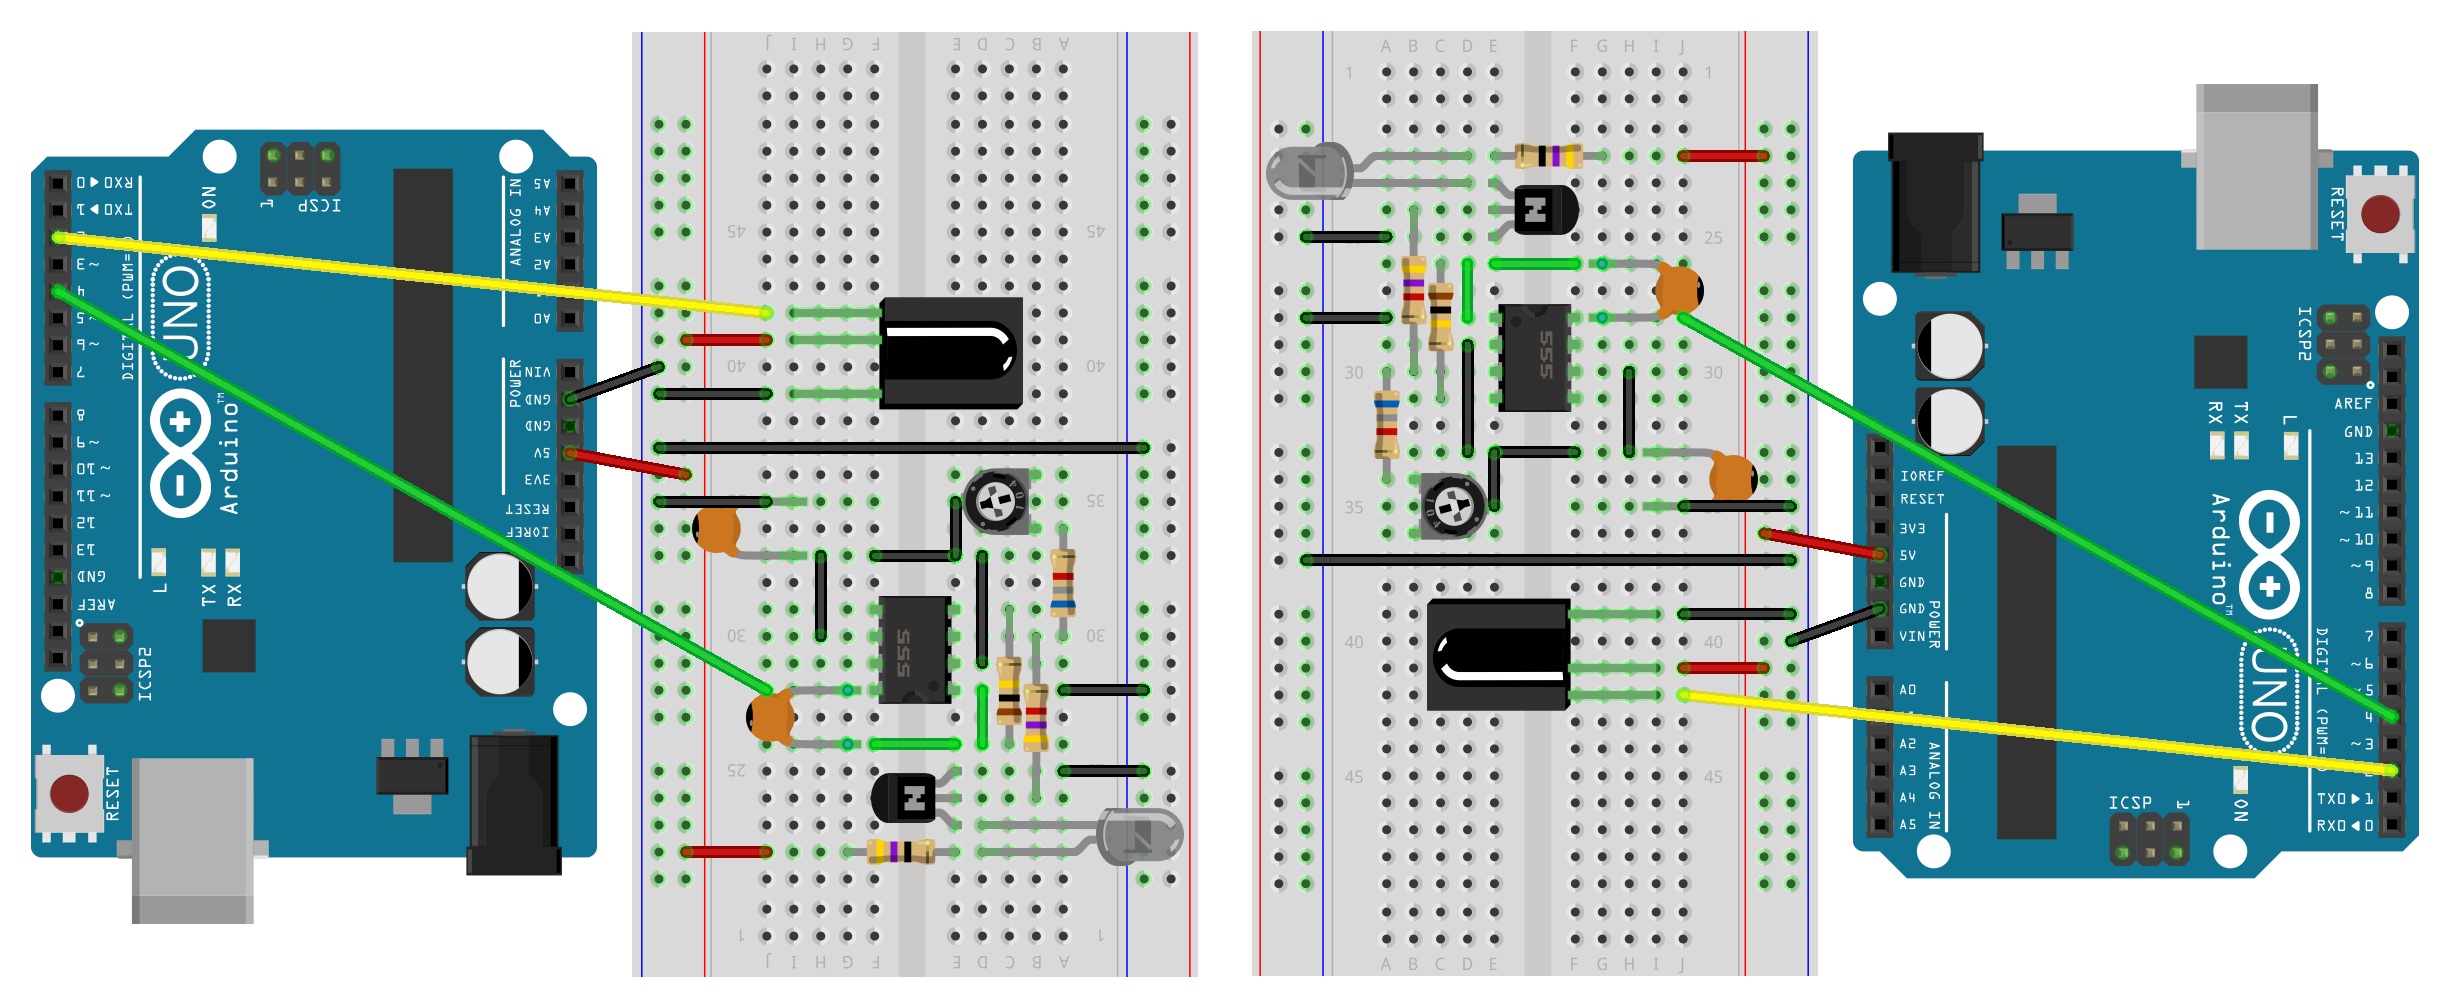
\includegraphics[width=\textwidth,height=\textheight,keepaspectratio]{res/wiring_scheme.png}

\subsection{Seven-segment display}
\label{sec:seven-segment}

In addition to the on-screen display, there is a seven segment display that can
show the numbers 0, 1, 2 and 3. During the game the local player's lives are
shown. While in the menu it will show the local player id.

Because there aren’t 7 pins left on the Arduino, a 4511 decoder chip is used to
control it. The chip has 4 input pins, which can be controlled as if counting
in binary: with all four pins low the display shows a 0, with only input A
(connected to pin A0) high a 1, with only input B (connected to pin A1) high a
2 and with both A and B high a 3.

Since the player only has 3 lives and player id is only 1 or 2, input C (adding
4) and input D (adding 8) have been soldered to the ground. That means the
display can show 4 numbers, 0, 1, 2 and 3, with only 2 of the Arduino’s output
pins.

The chip’s 7 output pins are connected, through a 330 ohm resistor each, to
a segment of the display.

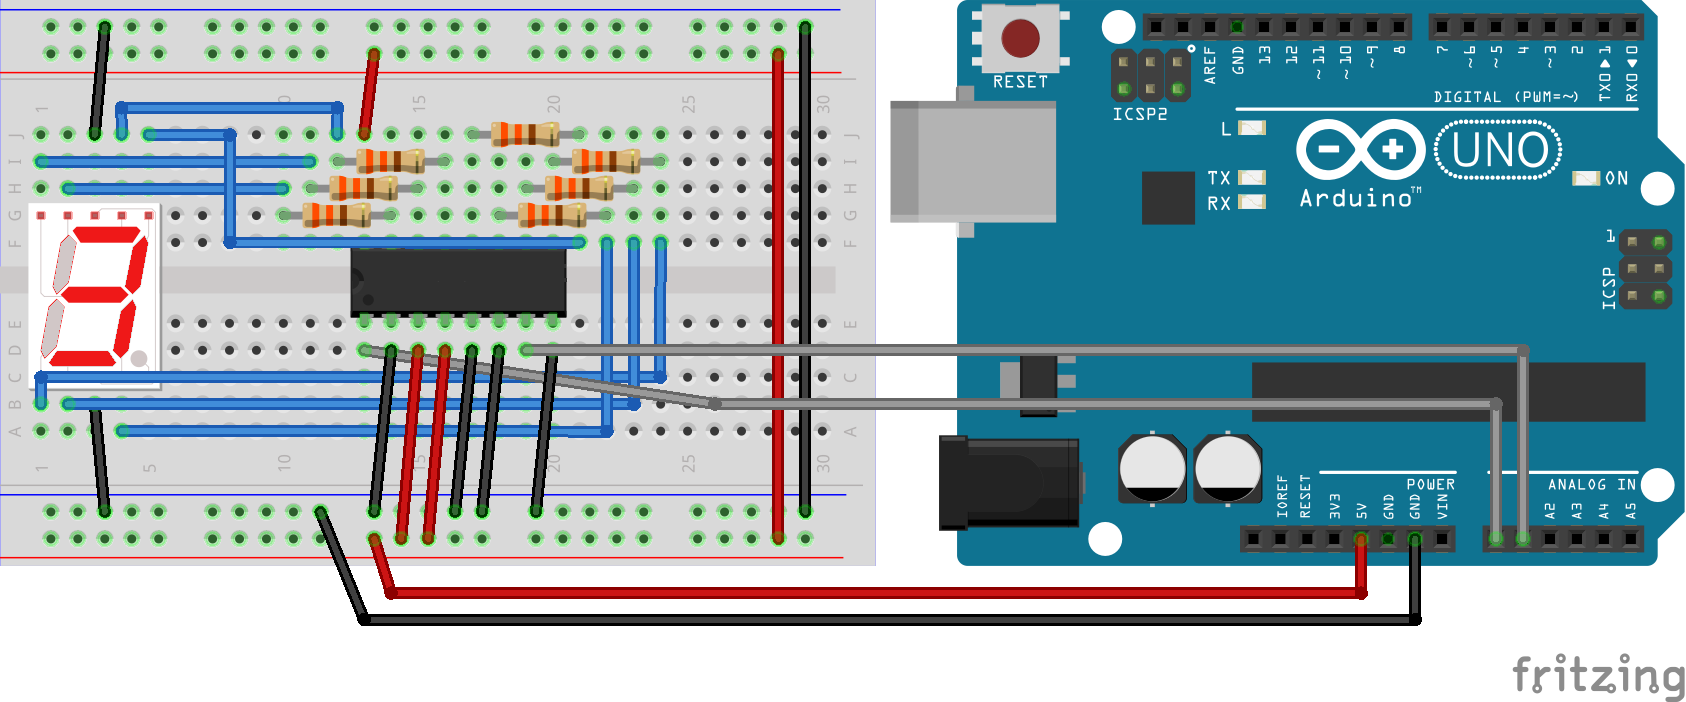
\includegraphics[width=\textwidth,height=\textheight,keepaspectratio]{res/seven-segment.png}

\subsection{Potentiometer}
\label{sec:potentiometer}

The brightness of the LCD screen is configurable by turning the handle of a
connected potentiometer. The potentiometer is connected to one of the Arduino's
analog input pins (pin A3), the input signal of which is measured by the
Arduino's Analog Digital Converter.

The ADC is configured to automatically trigger after each finished conversion,
allowing the game to just read the measured value whenever necessary without
using any timers or interrupts.

The ADC is initialized through the function \texttt{init\_brightness\_control},
which is called during initialization of the LCD display. Each render iteration
then calls the function \texttt{update\_lcd\_brightness}, which uses
\texttt{brightness\_control\_brightness} to get the appropriate brightness
percentage. \texttt{brightness\_control\_brightness} divides the output of the
ADC by the constant \texttt{BRIGHTNESS\_CONTROL\_DIVISOR}, because the output
of the ADC is a 10-bit number and the brightness percentage needs to be a
number between 0 and 100. The maximum value of a 10-bit number is 1024, which
means we need to divide it by 10.24, but because that's not an integer division
we divide by 11 instead.

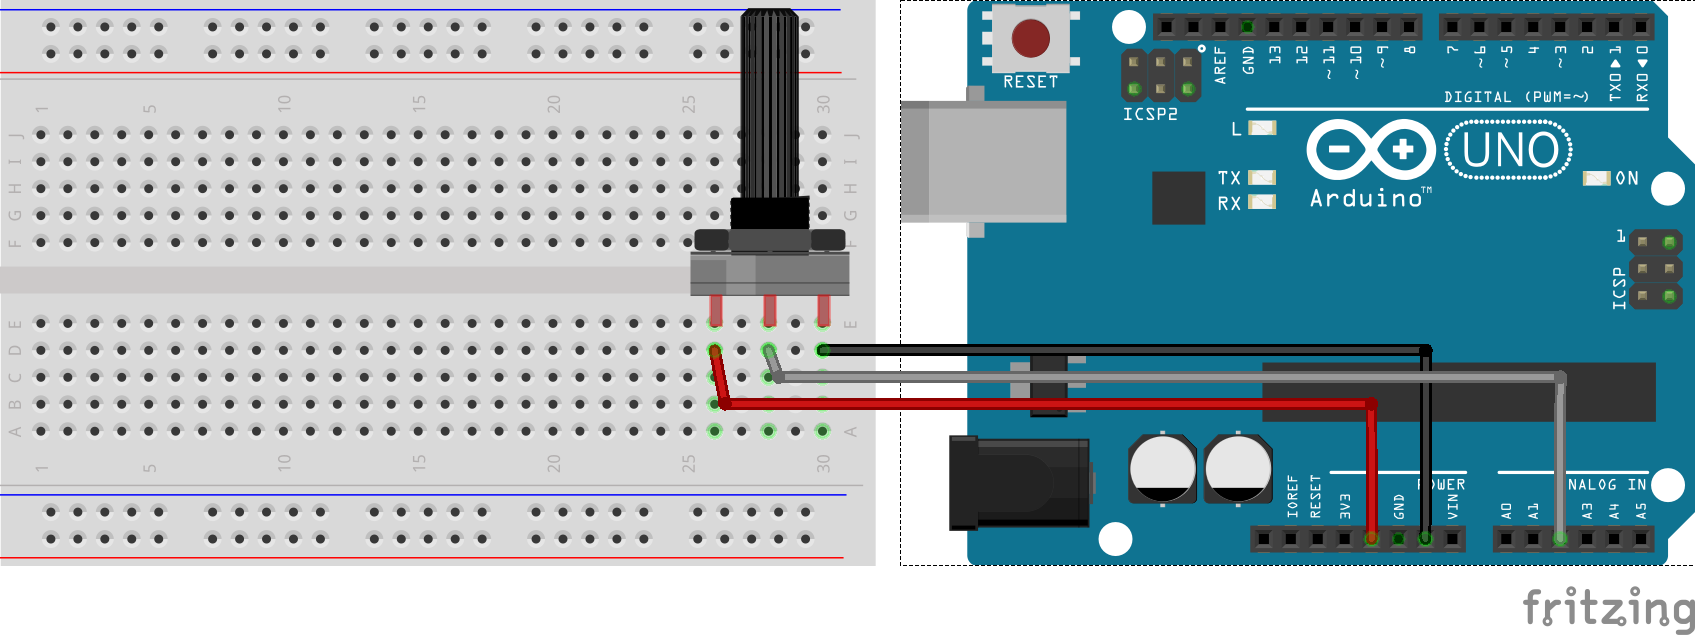
\includegraphics[width=\textwidth,height=\textheight,keepaspectratio]{res/potentiometer.png}

\subsection{Nunchuck}
\label{sec:nunchuck}

The nunchuck is connected to the 3.3V and a ground pin to provide power. The
other two wires are connected to pin A4 and A5, wich are the ports for I²C
communication.

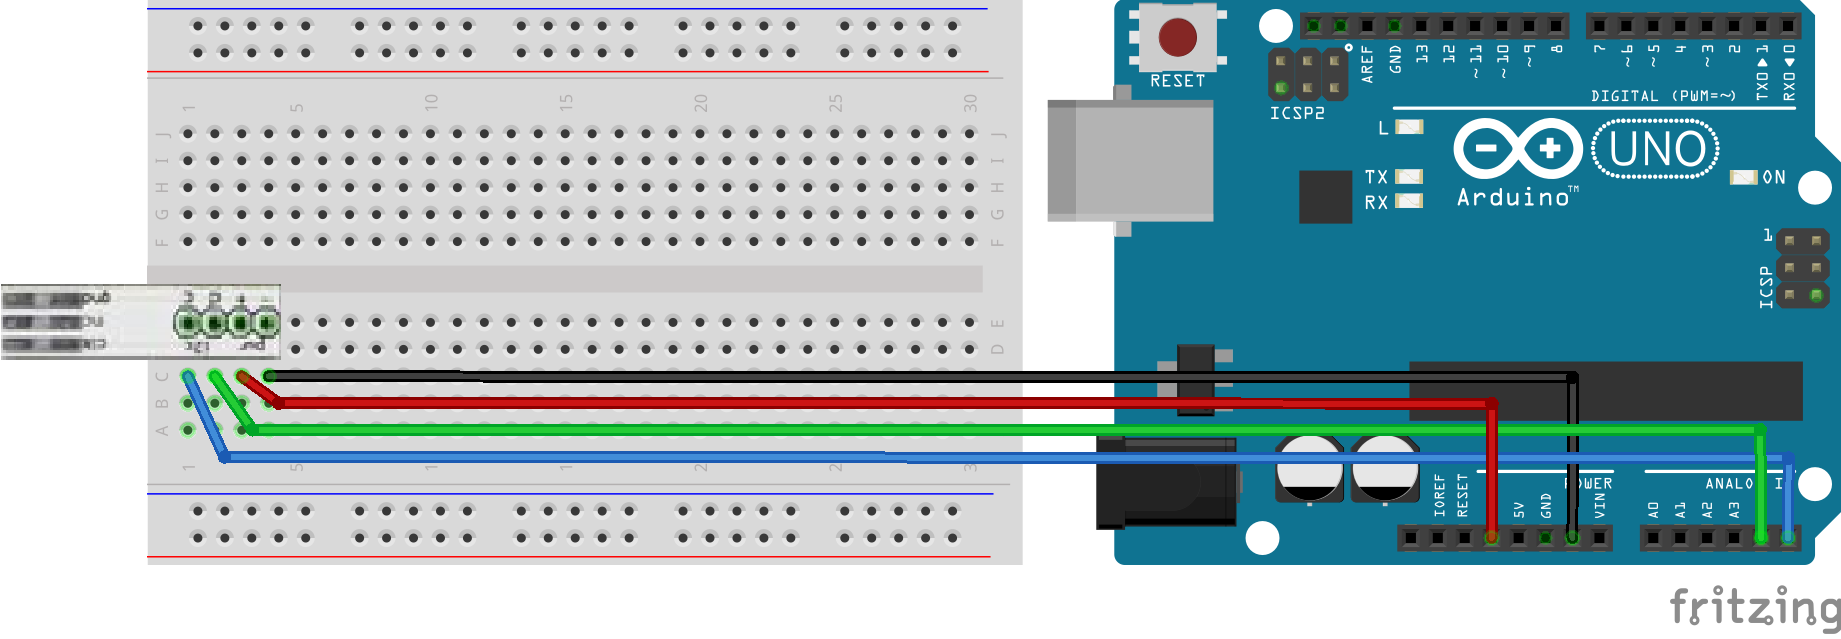
\includegraphics[width=\textwidth,height=\textheight,keepaspectratio]{res/nunchuck.png}

\subsection{LCD}
\label{sec:lcd}

The game is displayed on a Watterott MI0283QT-9 TFT-LCD\cite{mi0283qt9}\@. This
display is connected to the Arduino through an mSD-Shield\cite{msd-shield}. It
uses several pins, namely Arduino pins 6, 7, 8, 9, 11, 12, 13. These correspond
to pins PD6, PD7, PB0, PB1, PB3, PB4 and PB5 of the ATmega chip.
